%%%%%%%%%%%%%%%%%%%%%%%%%%%%%%%%%%%%%%%%%%%%%%%%%%%%%%%%%%%%%%%%%%%%%
%%                                                                 %%
%% Please do not use \input{...} to include other tex files.       %%
%% Submit your LaTeX manuscript as one .tex document.              %%
%%                                                                 %%
%% All additional figures and files should be attached             %%
%% separately and not embedded in the \TeX\ document itself.       %%
%%                                                                 %%
%%%%%%%%%%%%%%%%%%%%%%%%%%%%%%%%%%%%%%%%%%%%%%%%%%%%%%%%%%%%%%%%%%%%%

%%\documentclass[referee,sn-basic]{sn-jnl}% referee option is meant for double line spacing

%%=======================================================%%
%% to print line numbers in the margin use lineno option %%
%%=======================================================%%

%%\documentclass[lineno,sn-basic]{sn-jnl}% Basic Springer Nature Reference Style/Chemistry Reference Style

%%======================================================%%
%% to compile with pdflatex/xelatex use pdflatex option %%
%%======================================================%%

%%\documentclass[pdflatex,sn-basic]{sn-jnl}% Basic Springer Nature Reference Style/Chemistry Reference Style

%%\documentclass[sn-basic]{sn-jnl}% Basic Springer Nature Reference Style/Chemistry Reference Style
%%\documentclass[sn-mathphys]{sn-jnl}% Math and Physical Sciences Reference Style
%%\documentclass[sn-aps]{sn-jnl}% American Physical Society (APS) Reference Style
%%\documentclass[sn-vancouver]{sn-jnl}% Vancouver Reference Style
%%\documentclass[sn-apa]{sn-jnl}% APA Reference Style
%%\documentclass[sn-chicago]{sn-jnl}% Chicago-based Humanities Reference Style
%%\documentclass[sn-standardnature]{sn-jnl}% Standard Nature Portfolio Reference Style
%%\documentclass[default]{sn-jnl}% Default
\documentclass[default,iicol]{sn-jnl}% Default with double column layout

%%%% Standard Packages
%%<additional latex packages if required can be included here>
\usepackage{xcolor}
\usepackage[colorlinks, linkcolor=blue, citecolor=pink]{hyperref}
\usepackage{url}
\usepackage{listings}
\usepackage{xcolor}      %代码着色宏包
\usepackage{CJK}
\usepackage{mathrsfs}

% add your local package settings here
\lstset{
    basicstyle=\tt,
    %行号
    numbers=left,
    rulesepcolor=\color{red!20!green!20!blue!20},
    escapeinside=``,
    xleftmargin=2em,xrightmargin=2em, aboveskip=1em,
    %背景框
    framexleftmargin=1.5mm,
    frame=shadowbox,
    %背景色
    backgroundcolor=\color[RGB]{245,245,244},
    %样式
    keywordstyle=\color{blue}\bfseries,
    identifierstyle=\bf,
    numberstyle=\color[RGB]{0,192,192},
    commentstyle=\it\color[RGB]{96,96,96},
    stringstyle=\rmfamily\slshape\color[RGB]{128,0,0},
    %显示空格
    showstringspaces=false
}

%%%%

%%%%%=============================================================================%%%%
%%%%  Remarks: This template is provided to aid authors with the preparation
%%%%  of original research articles intended for submission to journals published 
%%%%  by Springer Nature. The guidance has been prepared in partnership with 
%%%%  production teams to conform to Springer Nature technical requirements. 
%%%%  Editorial and presentation requirements differ among journal portfolios and 
%%%%  research disciplines. You may find sections in this template are irrelevant 
%%%%  to your work and are empowered to omit any such section if allowed by the 
%%%%  journal you intend to submit to. The submission guidelines and policies 
%%%%  of the journal take precedence. A detailed User Manual is available in the 
%%%%  template package for technical guidance.
%%%%%=============================================================================%%%%

\jyear{2021}%

%% as per the requirement new theorem styles can be included as shown below
\theoremstyle{thmstyleone}%
\newtheorem{theorem}{Theorem}%  meant for continuous numbers
%%\newtheorem{theorem}{Theorem}[section]% meant for sectionwise numbers
%% optional argument [theorem] produces theorem numbering sequence instead of independent numbers for Proposition
\newtheorem{proposition}[theorem]{Proposition}% 
%%\newtheorem{proposition}{Proposition}% to get separate numbers for theorem and proposition etc.

\theoremstyle{thmstyletwo}%
\newtheorem{example}{Example}%
\newtheorem{remark}{Remark}%

\theoremstyle{thmstylethree}%
\newtheorem{definition}{Definition}%

\raggedbottom
%%\unnumbered% uncomment this for unnumbered level heads

\graphicspath{{./graphs/}}

\begin{document}

\title[Article Title]{A Concurrent Membrane Computing Scheme}

%%=============================================================%%
%% Prefix	-> \pfx{Dr}
%% GivenName	-> \fnm{Joergen W.}
%% Particle	-> \spfx{van der} -> surname prefix
%% FamilyName	-> \sur{Ploeg}
%% Suffix	-> \sfx{IV}
%% NatureName	-> \tanm{Poet Laureate} -> Title after name
%% Degrees	-> \dgr{MSc, PhD}
%% \author*[1,2]{\pfx{Dr} \fnm{Joergen W.} \spfx{van der} \sur{Ploeg} \sfx{IV} \tanm{Poet Laureate} 
%%                 \dgr{MSc, PhD}}\email{iauthor@gmail.com}
%%=============================================================%%

\author*{\fnm{Hao} \sur{Bai*} \dgr{Ph.D}}\email{Haob.19@intl.zju.edu.cn}

\author{\fnm{Keyi} \sur{Shen}}\email{Keyi.19@intl.zju.edu.cn}
\equalcont{These authors contributed equally to this work.}

\author{\fnm{Arko} \sur{Dey}}\email{Arko.18@intl.zju.edu.cn}
\equalcont{These authors contributed equally to this work.}


\affil{\orgdiv{Electronic \& Computing Engineering Department}, \orgname{Zhejiang University - University of Illinois at Urbana-Champaign}, \orgaddress{\street{Haizhou East Road}, \city{Haining}, \postcode{314400}, \state{Zhejiang}, \country{China}}}

%\affil[2]{\orgdiv{Department}, \orgname{Organization}, \orgaddress{\street{Street}, \city{City}, \postcode{10587}, \state{State}, \country{Country}}}

%\affil[3]{\orgdiv{Department}, \orgname{Organization}, \orgaddress{\street{Street}, \city{City}, \postcode{610101}, \state{State}, \country{Country}}}

%%==================================%%
%% sample for unstructured abstract %%
%%==================================%%

\abstract{This part will be finished soon.}

%%================================%%
%% Sample for structured abstract %%
%%================================%%

% \abstract{\textbf{Purpose:} The abstract serves both as a general introduction to the topic and as a brief, non-technical summary of the main results and their implications. The abstract must not include subheadings (unless expressly permitted in the journal's Instructions to Authors), equations or citations. As a guide the abstract should not exceed 200 words. Most journals do not set a hard limit however authors are advised to check the author instructions for the journal they are submitting to.
% 
% \textbf{Methods:} The abstract serves both as a general introduction to the topic and as a brief, non-technical summary of the main results and their implications. The abstract must not include subheadings (unless expressly permitted in the journal's Instructions to Authors), equations or citations. As a guide the abstract should not exceed 200 words. Most journals do not set a hard limit however authors are advised to check the author instructions for the journal they are submitting to.
% 
% \textbf{Results:} The abstract serves both as a general introduction to the topic and as a brief, non-technical summary of the main results and their implications. The abstract must not include subheadings (unless expressly permitted in the journal's Instructions to Authors), equations or citations. As a guide the abstract should not exceed 200 words. Most journals do not set a hard limit however authors are advised to check the author instructions for the journal they are submitting to.
% 
% \textbf{Conclusion:} The abstract serves both as a general introduction to the topic and as a brief, non-technical summary of the main results and their implications. The abstract must not include subheadings (unless expressly permitted in the journal's Instructions to Authors), equations or citations. As a guide the abstract should not exceed 200 words. Most journals do not set a hard limit however authors are advised to check the author instructions for the journal they are submitting to.}

\keywords{Chipyard, Gemmini, Transformer, System on Chip, Accelerator, Co-processor}

%%\pacs[JEL Classification]{D8, H51}

%%\pacs[MSC Classification]{35A01, 65L10, 65L12, 65L20, 65L70}

\maketitle

\section{Introduction}\label{sec1}


\section{Acknowledgements}\label{sec7}
We need to sincerely thank Professor K.D. Schewe.

\bibliographystyle{IEEEtran}
\bibliography{reference.bib}

\newpage 
\onecolumn
\begin{appendices}

\section{Code Space}\label{secA}
\subsection{The code for transformer multiplication and calculation of matrix Q,K,V.}\label{secA1}

\lstset{language=C}
\begin{lstlisting}
for (int count = 0; count < n_head; count++)
  {
    tiled_matmul_auto(wordNum, weightDim, wordDim,
                      (elem_t *)word_vector, 
                      (elem_t *)q_mats[count], NULL, 
                      (elem_t *)z_qs[count],
                      wordDim, weightDim, 
                      weightDim, weightDim,
                      MVIN_SCALE_IDENTITY, 
                      MVIN_SCALE_IDENTITY, 
                      MVIN_SCALE_IDENTITY,
                      NO_ACTIVATION, ACC_SCALE_IDENTITY, 
                      0, false,
                      false, false,
                      false, false,
                      3,
                      accel_type);
    tiled_matmul_auto(wordNum, weightDim, wordDim,
                      (elem_t *)word_vector, 
                      (elem_t *)k_mats[count], NULL, 
                      (elem_t *)z_ks[count],
                      wordDim, weightDim, 
                      weightDim, weightDim,
                      MVIN_SCALE_IDENTITY, 
                      MVIN_SCALE_IDENTITY, 
                      MVIN_SCALE_IDENTITY,
                      NO_ACTIVATION, ACC_SCALE_IDENTITY, 
                      0, false,
                      false, false,
                      false, false,
                      3,
                      accel_type);
    tiled_matmul_auto(wordNum, weightDim, wordDim,
                      (elem_t *)word_vector, 
                      (elem_t *)v_mats[count], NULL, 
                      (elem_t *)z_vs[count],
                      wordDim, weightDim, 
                      weightDim, weightDim,
                      MVIN_SCALE_IDENTITY, 
                      MVIN_SCALE_IDENTITY, 
                      MVIN_SCALE_IDENTITY,
                      NO_ACTIVATION, 
                      ACC_SCALE_IDENTITY, 
                      0, false,
                      false, false,
                      false, false,
                      3,
                      accel_type);
  }


\end{lstlisting}

\subsection{The code for the exponential function mentioned in the Softmax calculation part.}\label{secA2}
\begin{lstlisting}
float my_exp(elem_t number)
{
  // float exp;
  // a is the slope
  float slope[24] = {0.006737946999085467, 0.0717489450711988, 
  0.13736897328580006, 0.20417102465724862, 0.27276942684711947,
  0.34384344502557984, 0.41816603105197925, 0.49664045641486215, 
  0.580348760164344, 0.6706178960296387, 0.7691126983842523, 
  0.8779702723670761, 1.0000000000000004, 1.1389907283579461, 
  1.3001995703630875, 1.4911621147011624, 1.7231018116017323, 
  2.0135290773908743, 2.39139462735484, 2.9083003165164474, 
  3.666100015528776, 4.897854637692817, 7.279664221697798, 
  13.937487150614775};
  // b is the inter
  float x0[24] = {-5, -3.38975777788707, -2.274768975664783, 
  -1.773836174919944, -1.4369560632507996, -1.1788714089484582, 
  -0.9665265685144582, -0.7834156082000947, -0.6199855288515437, 
  -0.4701006376974108, -0.3294748672686874, -0.19487414204749406, 
  -0.06366558341604925, 0.0664754970873836, 0.19778114058929605, 
  0.3325900427376481, 0.4735679272763055, 0.6240101415956079, 
  0.7883219072584459, 0.9728773115664778, 1.187761027381711, 
  1.4508594080418584, 1.7998227092372945, 2.3442268793669405};
  float y0[24] = {0.3860500834856052, 0.017587673747372003, 
  0.0975869440730206, 0.1663995685965194, 0.23518072618265692, 
  0.30557832941474355, 0.37859171088297716, 0.45516249439975104, 
  0.5363284835993326, 0.6233139943480013, 0.7176201526404586, 
  0.821143279619808, 0.936340493578349, 1.066481574081782, 
  1.216037484611534, 1.391315961265941, 1.6015368417007017, 
  1.8607640937356675, 2.191610611655227, 2.632955413966755,
  3.257901792686428, 4.22244677011019, 5.931618293254853, 
  9.894697852690719};
  for (int i = 0; i < 24; i++)
  {
    if (number < x0[i])
    {
      if (i != 0)
      {
        return slope[i - 1] * (number - x0[i - 1]) + y0[i - 1];
      }
      else
      {
        return slope[0] * (number - x0[0]) + y0[0];
      }
    }
  }
  return slope[23] * (number - x0[23]) + y0[23];
}


\end{lstlisting}


\subsection{The code for the square root function mentioned in the layer normalization calculation part.}\label{secA3}
\begin{lstlisting}
float my_sqrt(elem_t number)
{
  float sqrt;
  // a is the slope
  float a[16] = {0.3549, 0.1470, 0.1128, 0.0951, 0.0838, 
  0.0758, 0.0697, 0.0648, 0.0609, 0.0576, 0.0548, 0.0523, 
  0.0502, 0.0483, 0.0466, 0.0451};
  // b is the inter
  float b[16] = {0, 2.8174, 3.9843, 4.8798, 5.6347, 6.2998, 
  6.9011, 7.4540, 7.9687, 8.4521, 8.9093, 9.3441, 9.7596, 
  10.1581, 10.5416, 10.9116};
  float step = 7.9438;
  for (int i = 0; i < 16; i++)
  {
    if ((step * i <= number) && (number < step * (i + 1)))
    {
      sqrt = a[i] * number + b[i];
      break;
    }
  }
}

\end{lstlisting}

\section{Big Graph Space}\label{secB}
%% Appendices may be used for helpful, supporting or essential material that would otherwise 
%% clutter, break up or be distracting to the text. Appendices can consist of sections, figures, 
%% tables and equations etc.

\begin{figure}[H]
	\begin{center}
		%\fbox{\rule{0pt}{2in} \rule{0.9\linewidth}{0pt}}
  		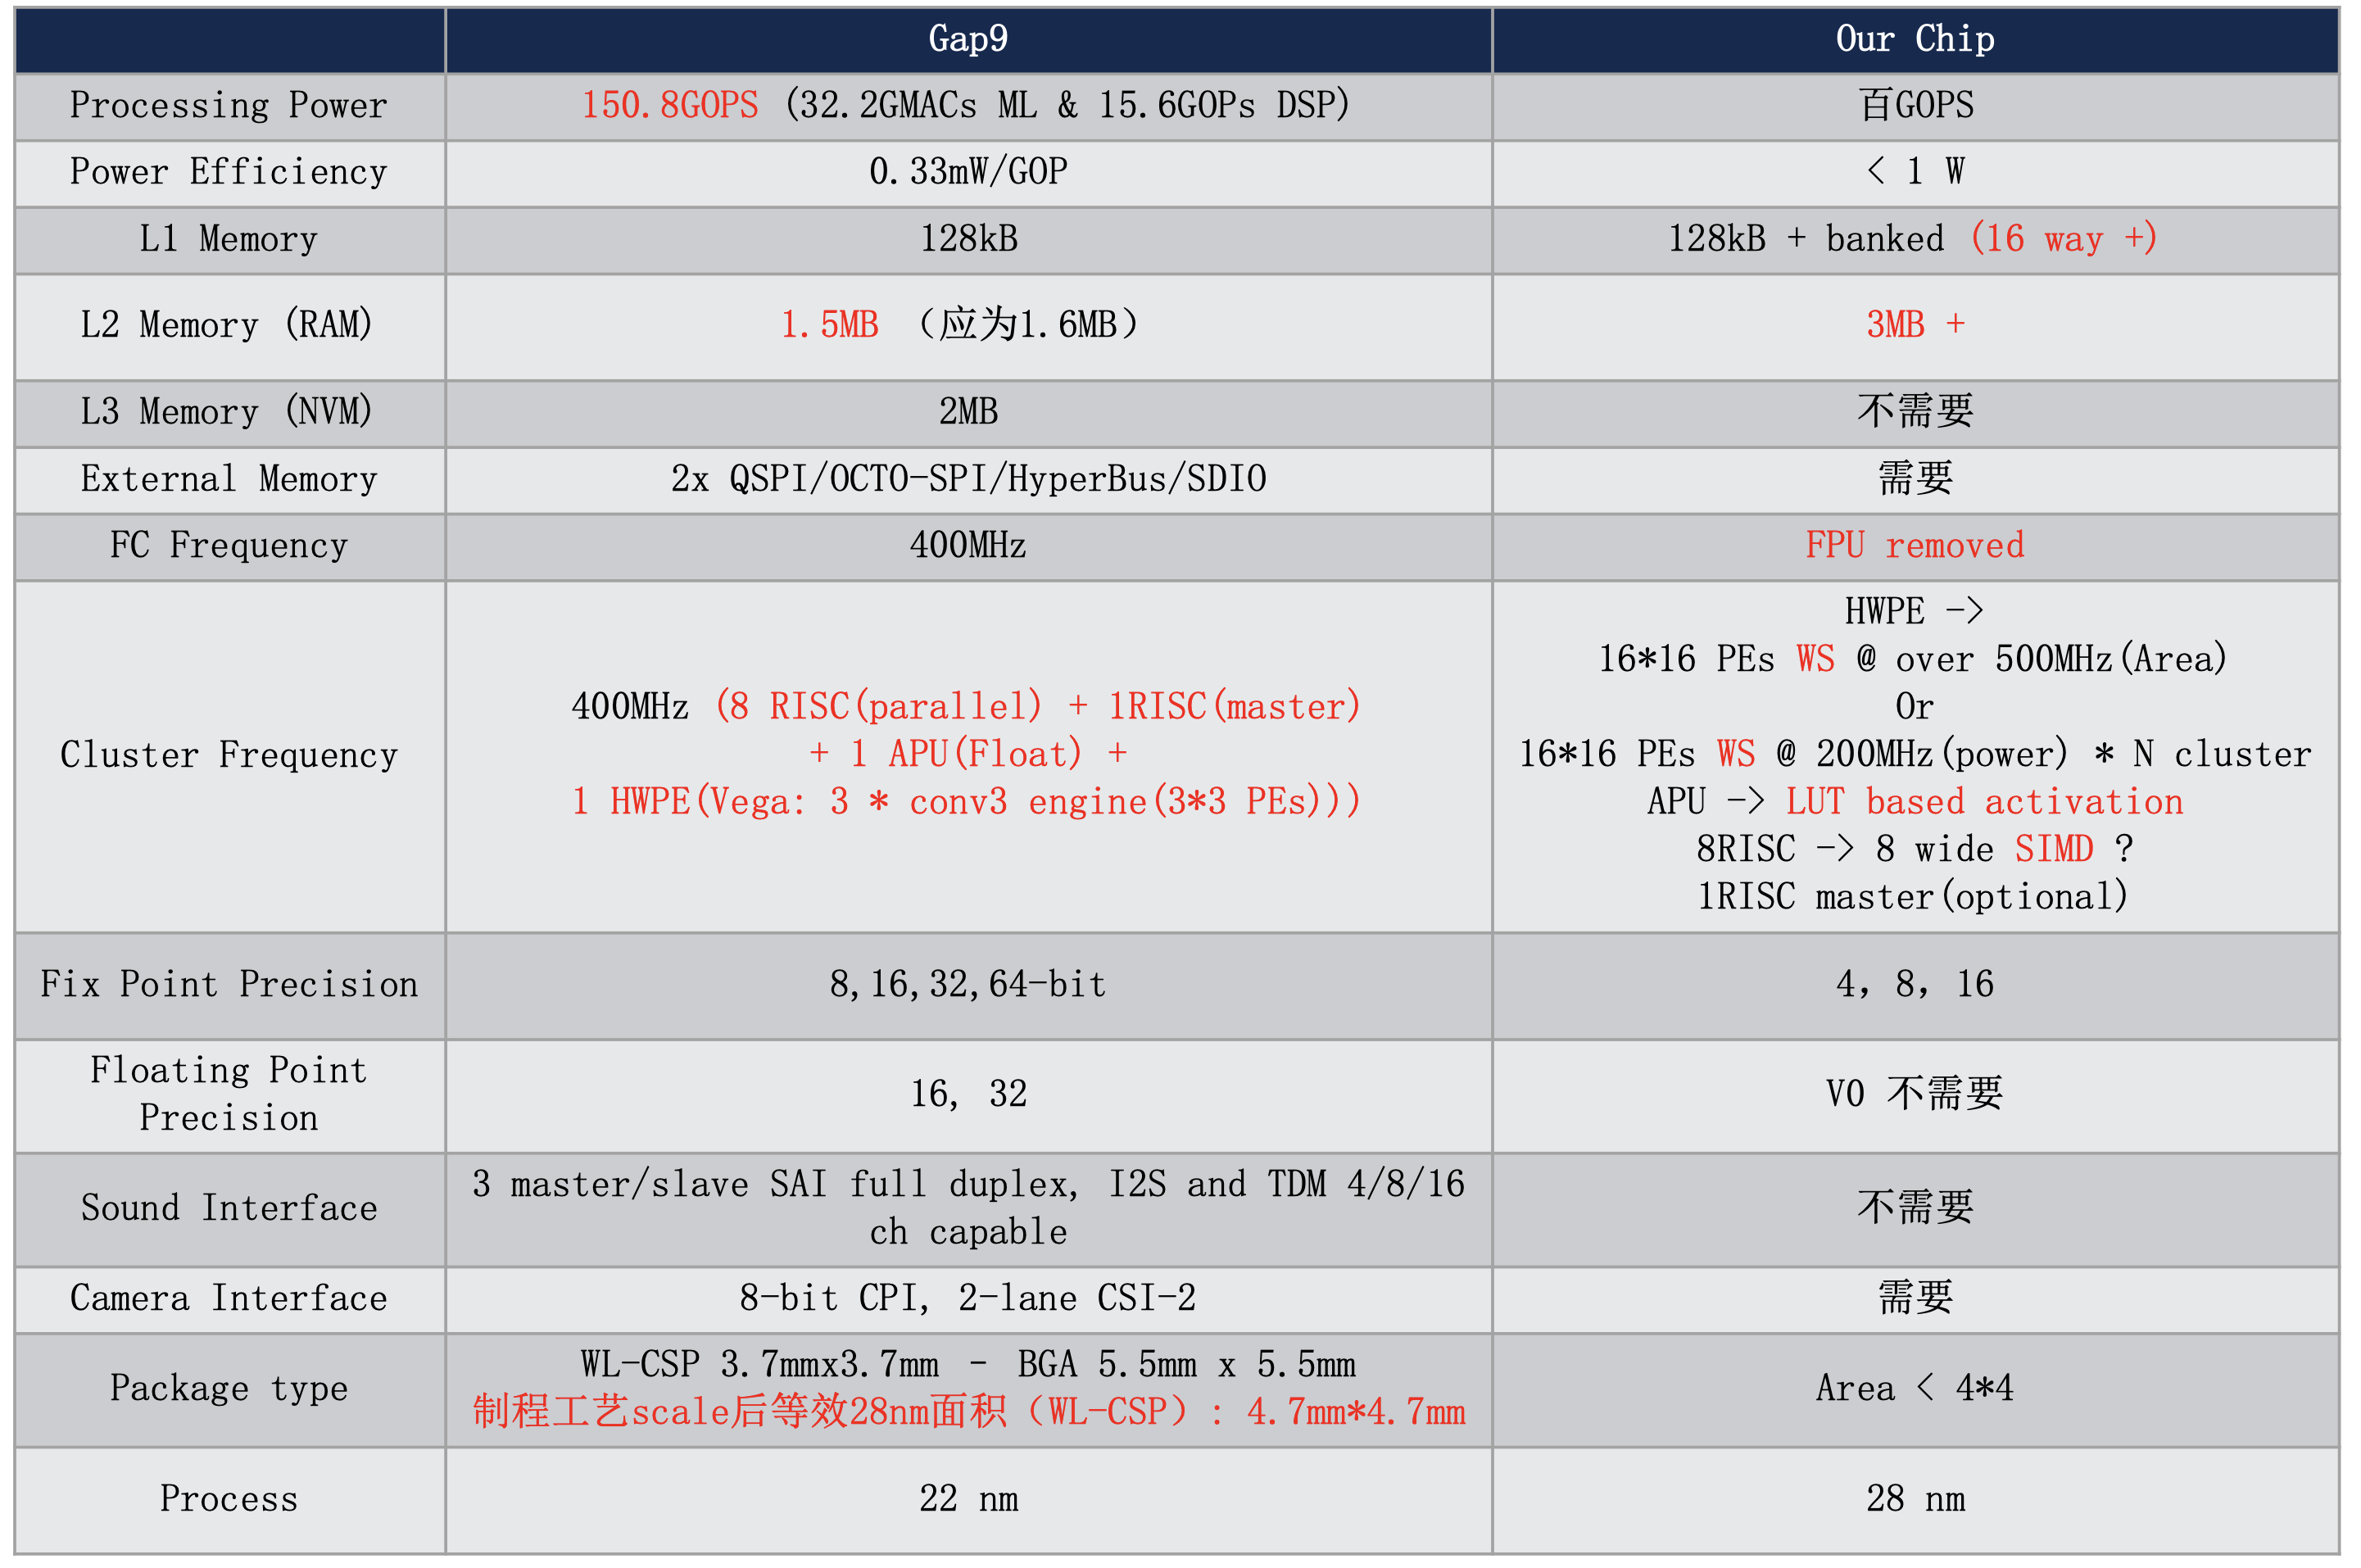
\includegraphics[width=1.0\linewidth]{Gap9andOurChip.png}
	\end{center}
   	\caption{The comparison of \textit{Gap 9} and our chip.}
	\label{fig:Gap_9_and_our_chip}
\end{figure}

\begin{figure}[H]
	\begin{center}
		%\fbox{\rule{0pt}{2in} \rule{0.9\linewidth}{0pt}}
  		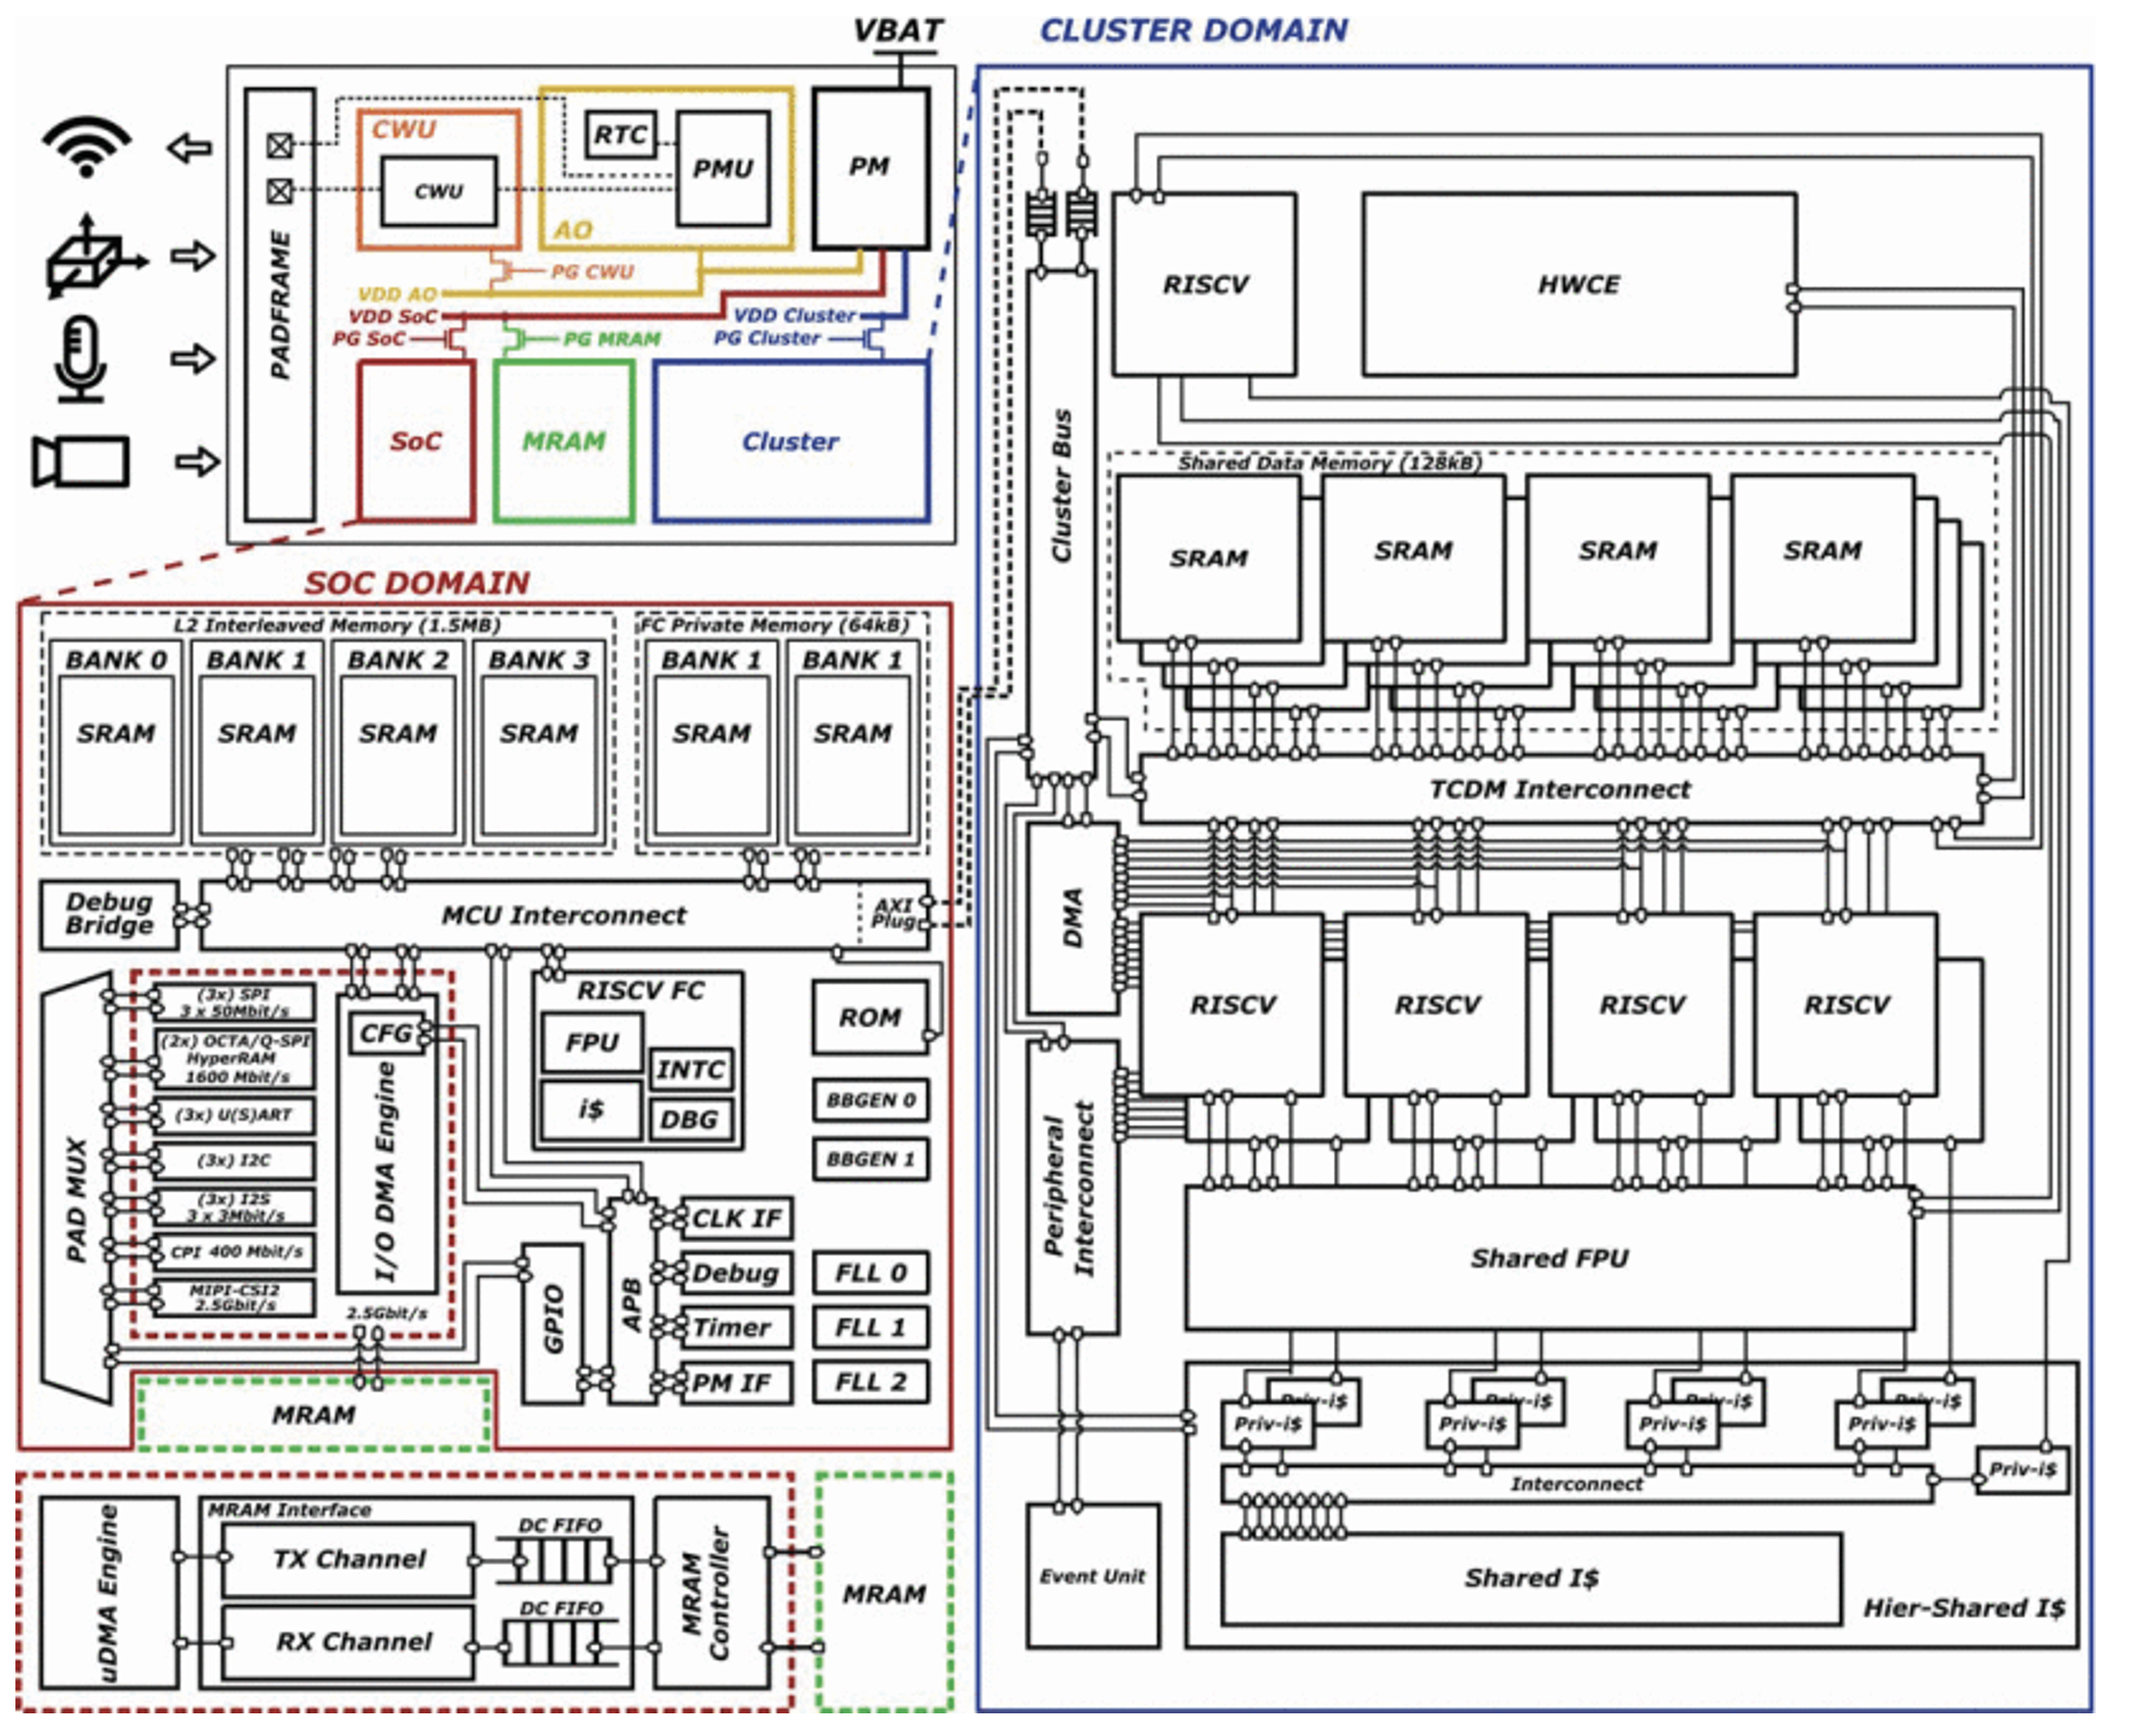
\includegraphics[width=1.0\linewidth]{SoC_original.png}
	\end{center}
   	\caption{The original SoC Layout.}
	\label{fig:SoC_original}
\end{figure}

\begin{figure}[H]
	\begin{center}
		%\fbox{\rule{0pt}{2in} \rule{0.9\linewidth}{0pt}}
  		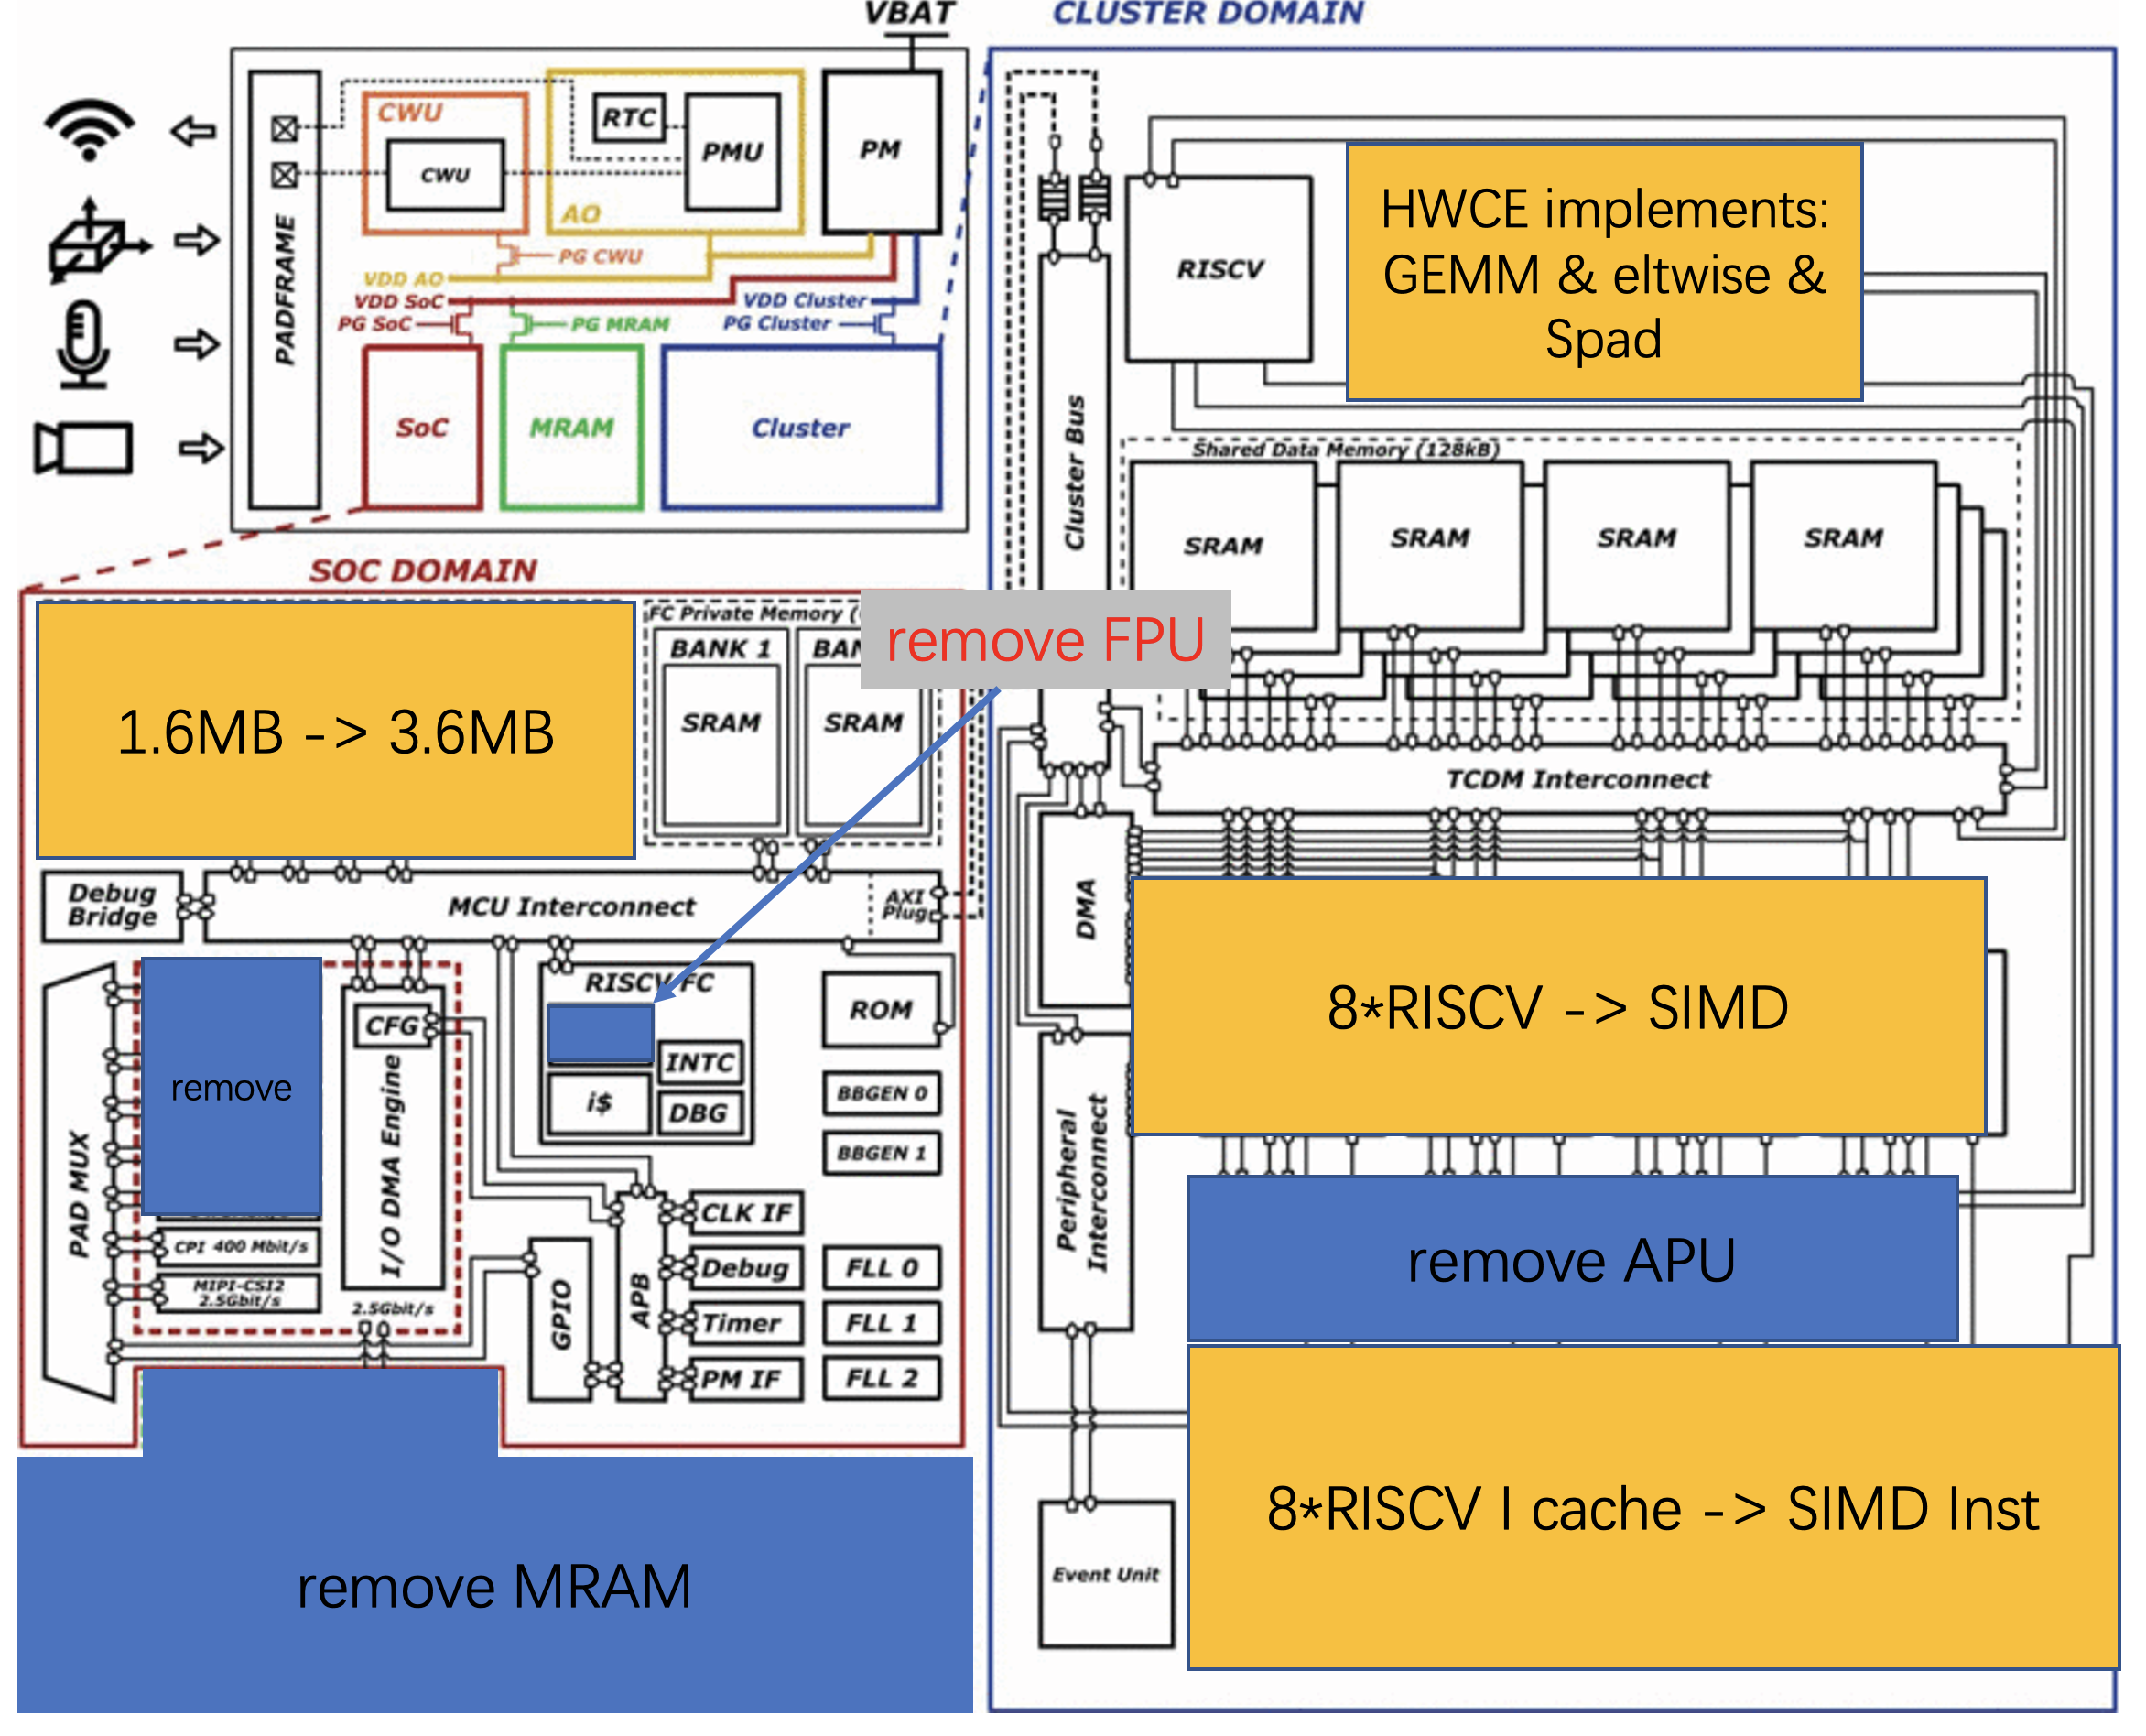
\includegraphics[width=1.0\linewidth]{SoC_new.png}
	\end{center}
   	\caption{Our design to refine the original SoC Layout.}
	\label{fig:SoC_new}
\end{figure}


\end{appendices}

%%===========================================================================================%%
%% If you are submitting to one of the Nature Portfolio journals, using the eJP submission   %%
%% system, please include the references within the manuscript file itself. You may do this  %%
%% by copying the reference list from your .bbl file, paste it into the main manuscript .tex %%
%% file, and delete the associated \verb+\bibliography+ commands.                            %%
%%===========================================================================================%%



%% if required, the content of .bbl file can be included here once bbl is generated
%%\input sn-article.bbl

%% Default %%
%\input sn-sample-bib.tex%

\end{document}
